
\chapter{Per-Category Mass Plots}
\label{appendix:mass_plots}

\begin{figure}[h!]
    \begin{center}
        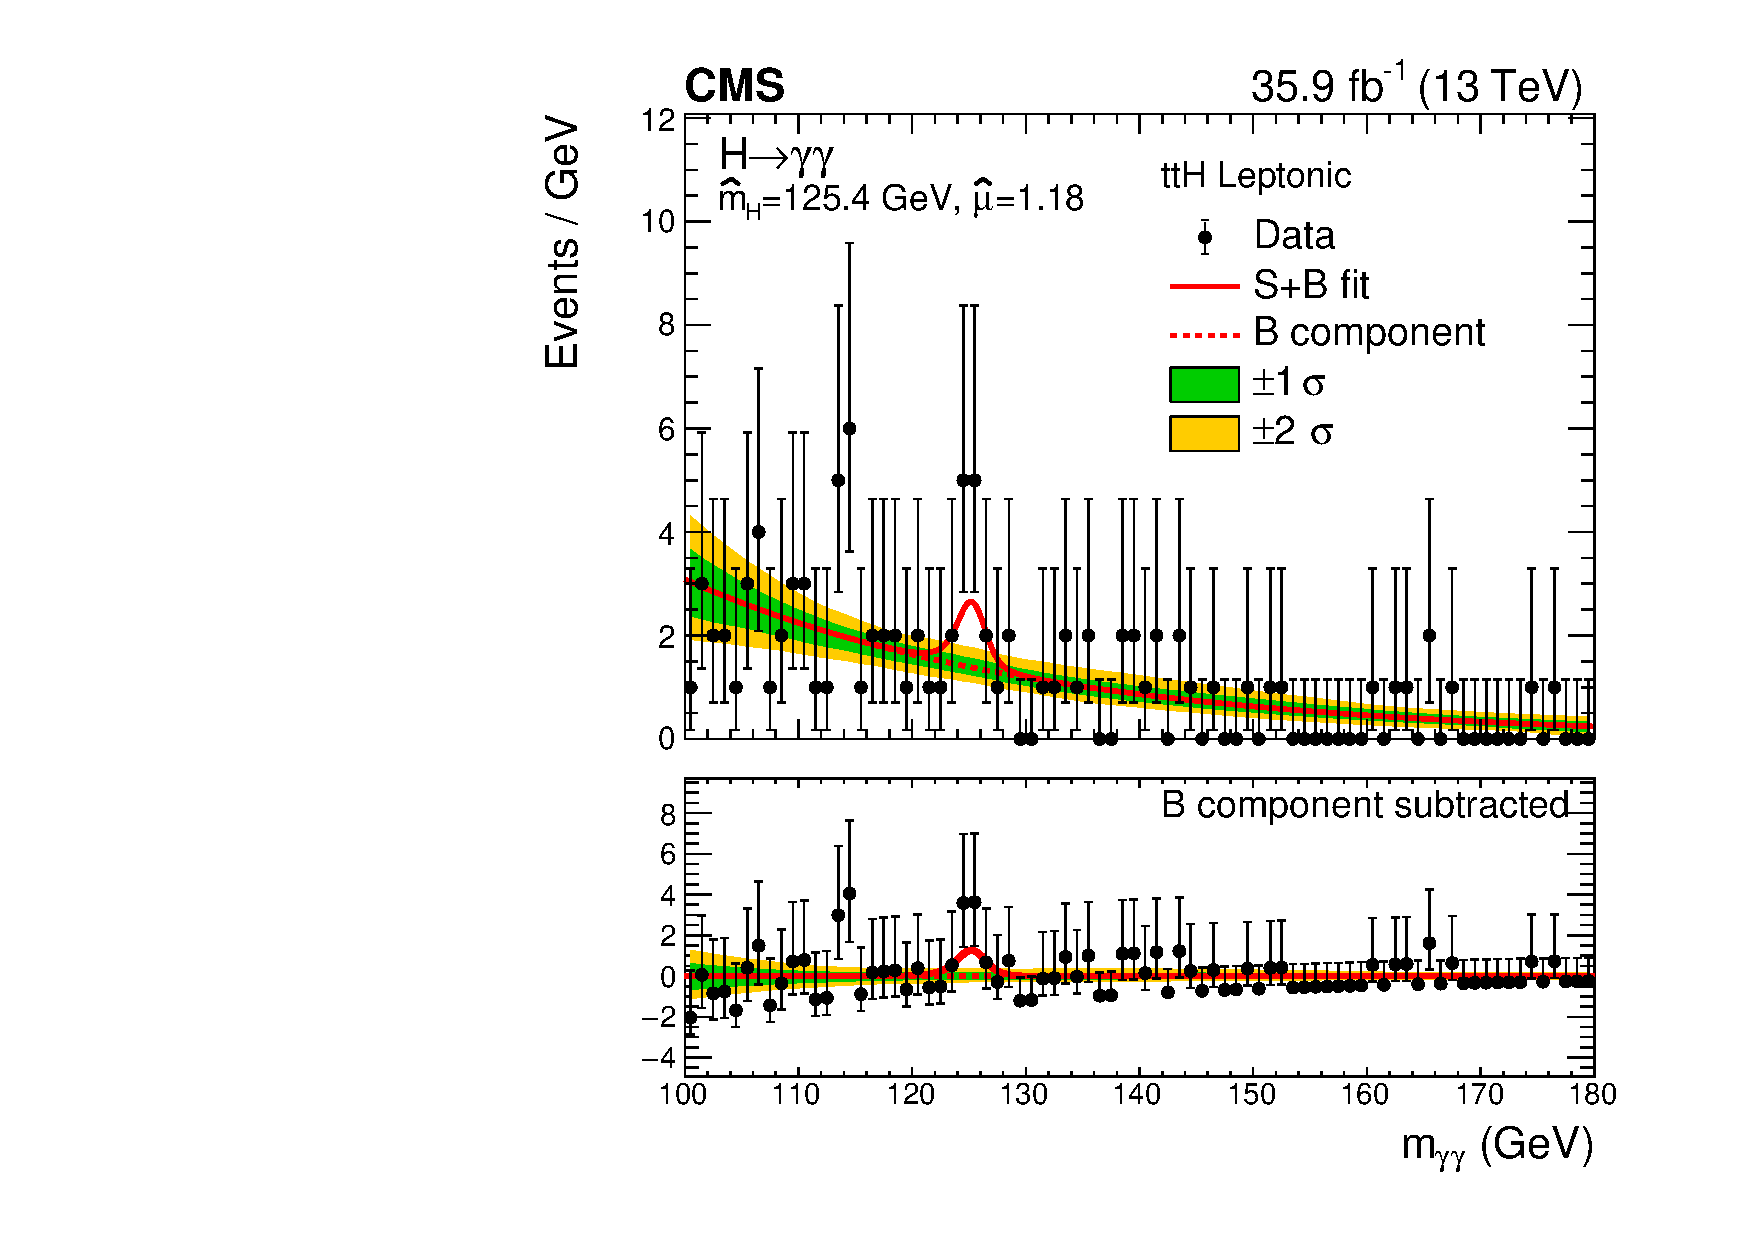
\includegraphics[width=0.49\textwidth]{figures/appendix_mass_plots/CMS-HIG-16-040_Figure_012-d.pdf}
        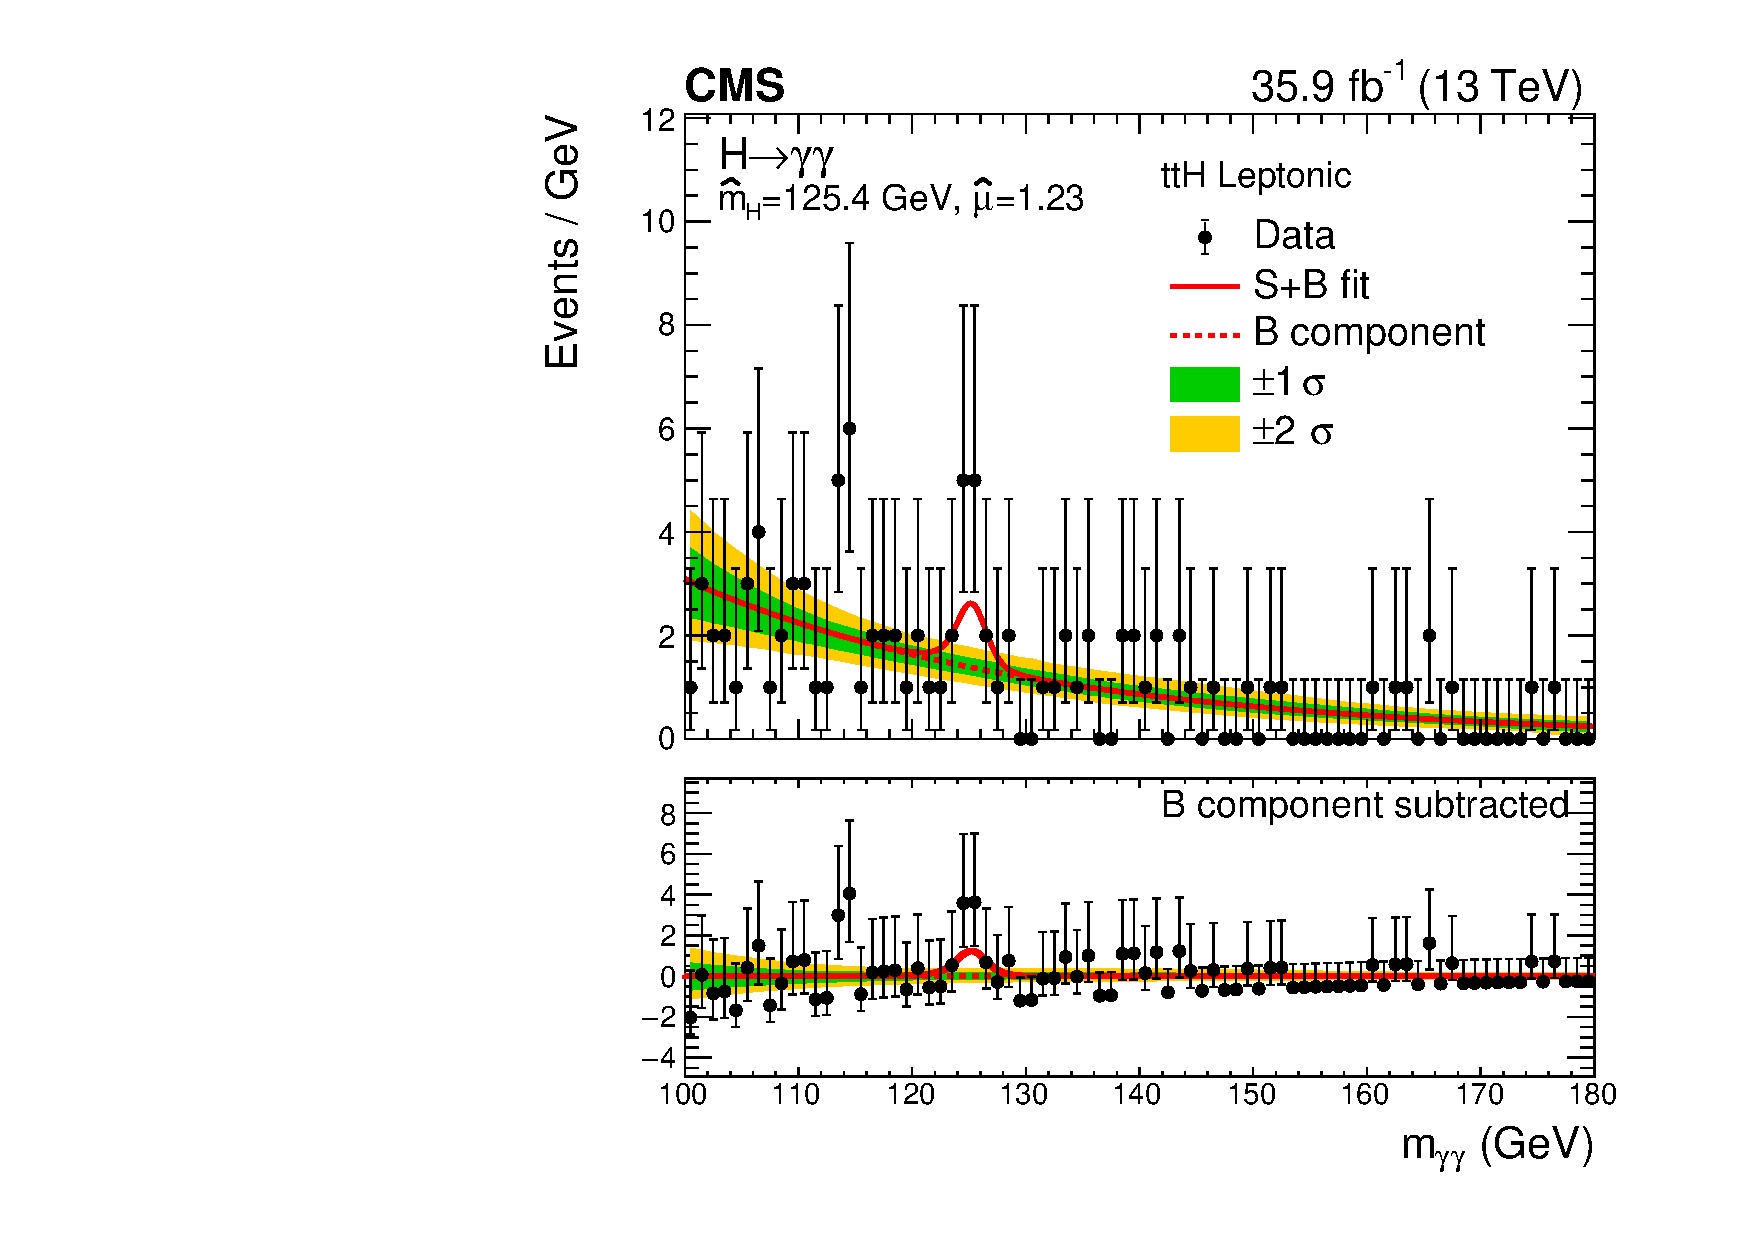
\includegraphics[width=0.49\textwidth]{figures/appendix_mass_plots/SBplots_jackWSnewTTHLeptonicTag_13TeV.pdf}
    \end{center}
    \begin{center}
        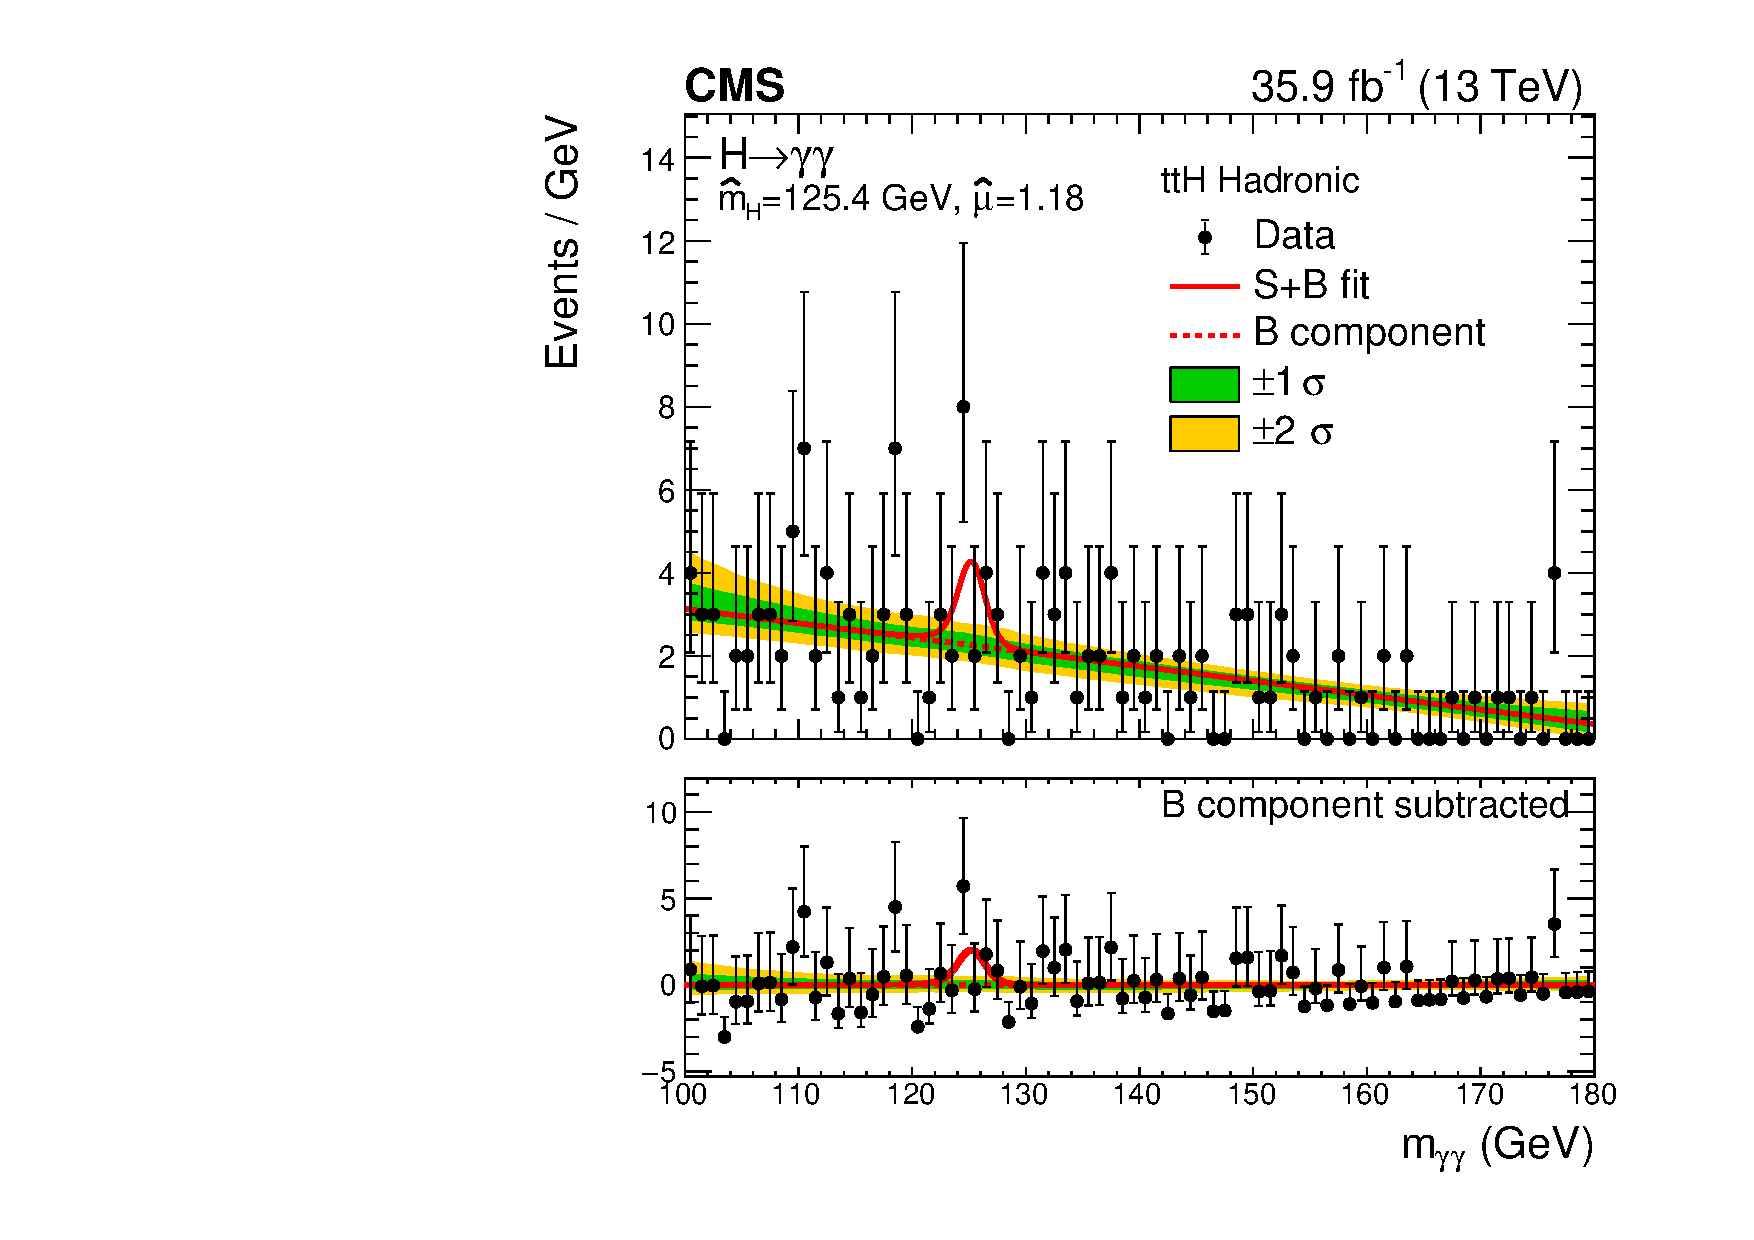
\includegraphics[width=0.49\textwidth]{figures/appendix_mass_plots/CMS-HIG-16-040_Figure_012-e.pdf}
        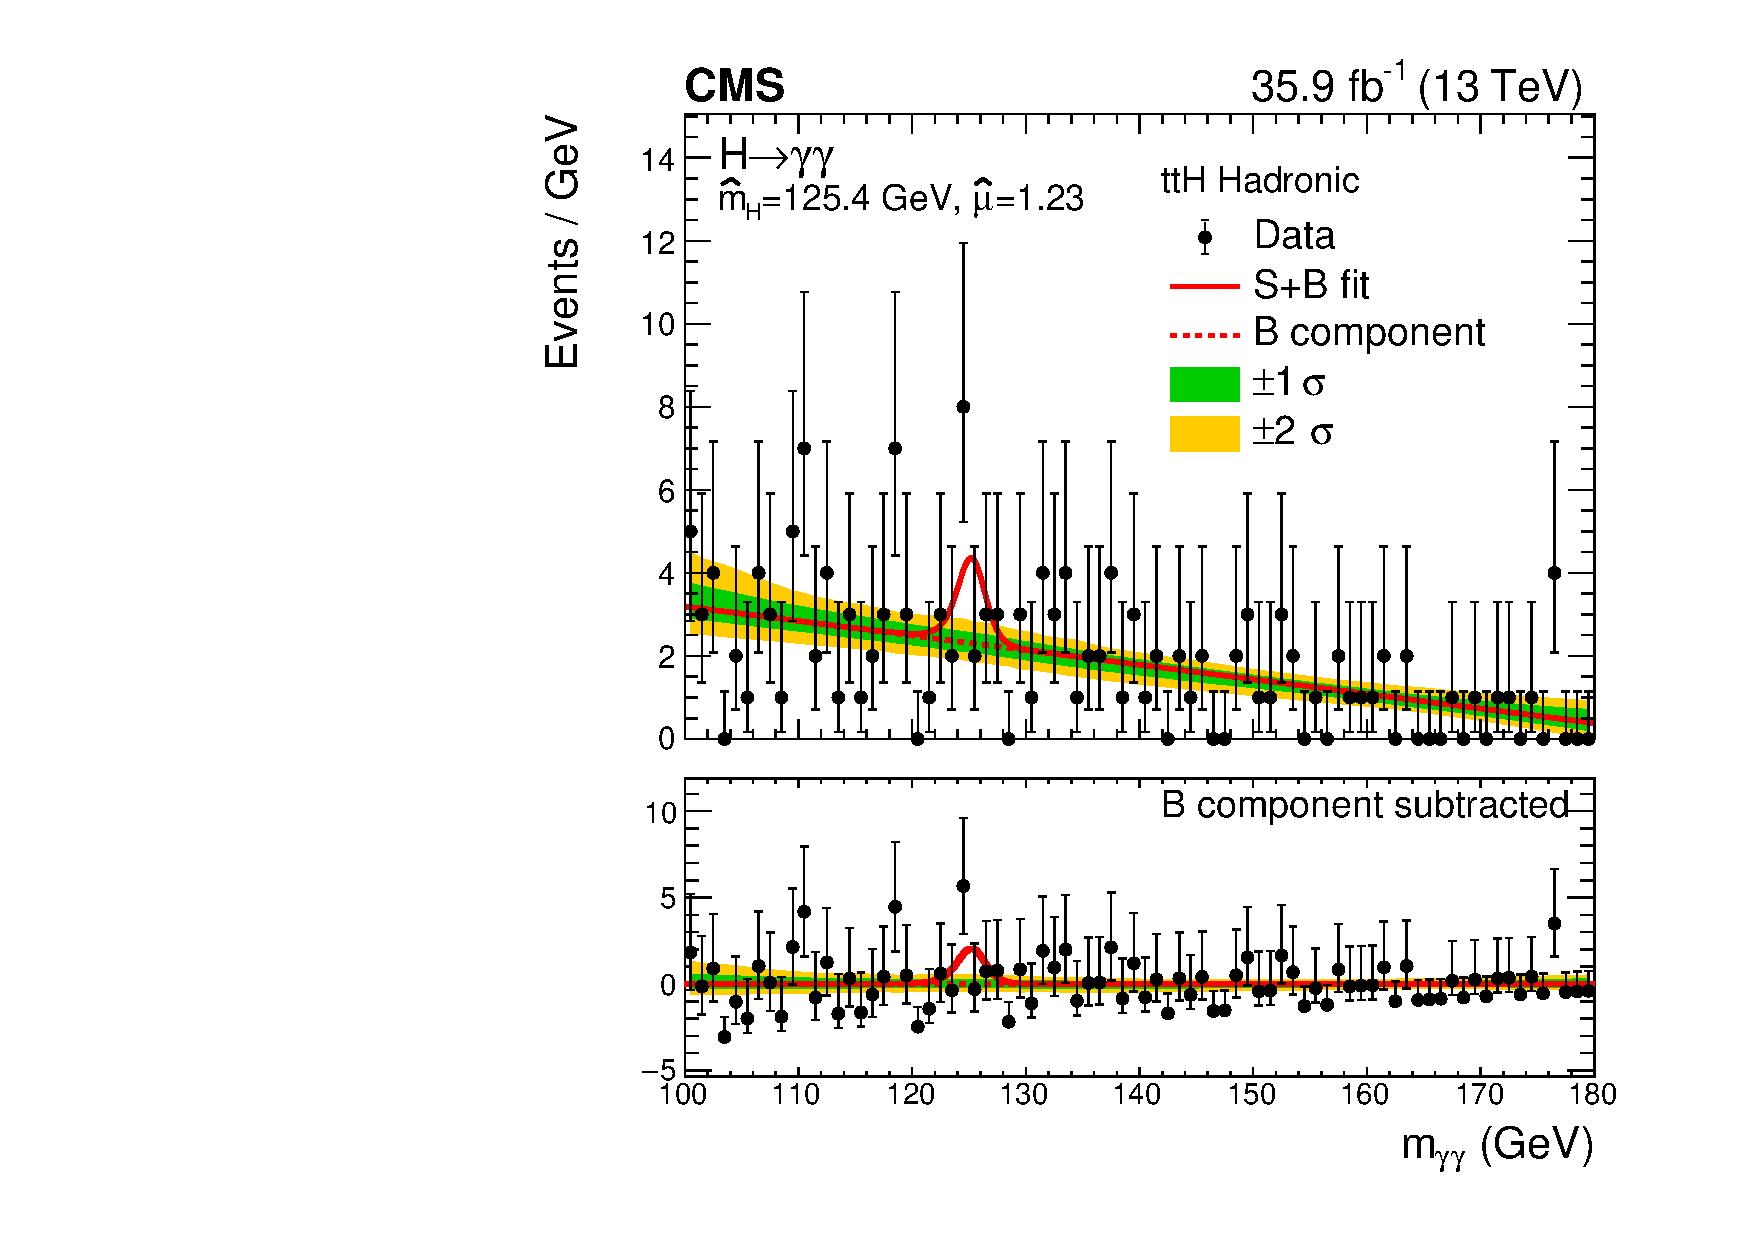
\includegraphics[width=0.49\textwidth]{figures/appendix_mass_plots/SBplots_jackWSnewTTHHadronicTag_13TeV.pdf}
    \end{center}
    \label{fig:app_mass_plots:tth}
    \caption{Mass plots of the \ttH tags. BDT-based VBF analysis is shown on the left on the left, DCNN on the right. These upstream tags are the same, as expected.}
\end{figure}


